

\tikzset{every picture/.style={line width=0.75pt}} %set default line width to 0.75pt        

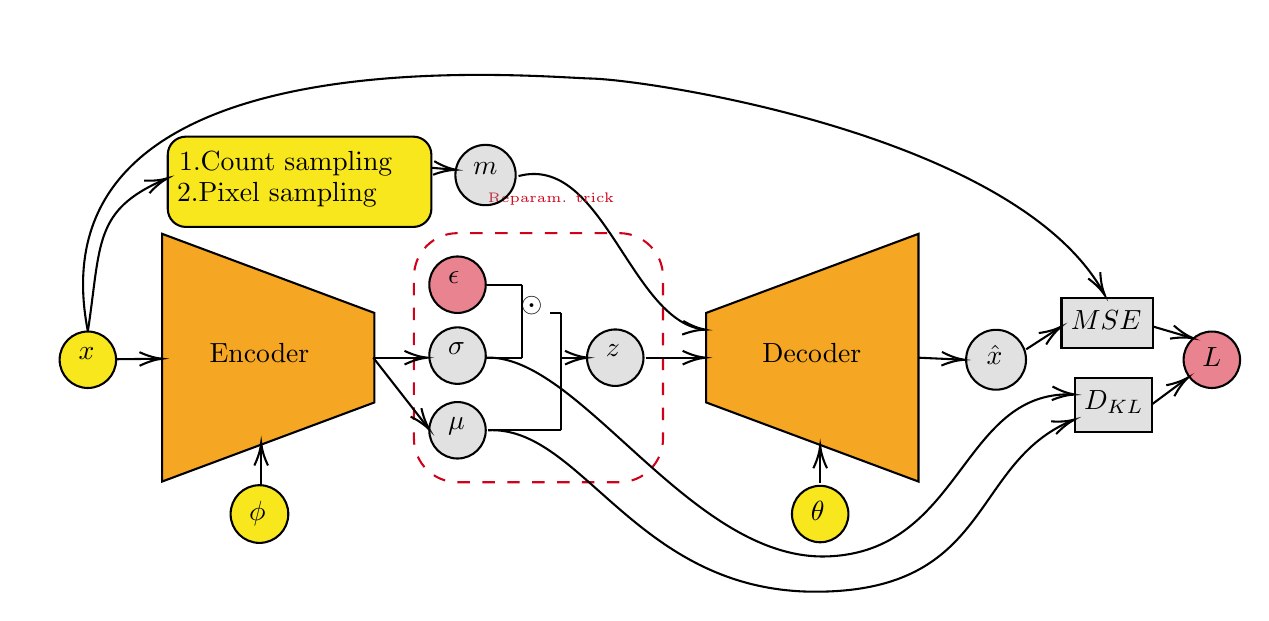
\begin{tikzpicture}[x=0.75pt,y=0.75pt,yscale=-1,xscale=1]
%uncomment if require: \path (0,300); %set diagram left start at 0, and has height of 300

%Shape: Trapezoid [id:dp4858077127891579] 
\draw  [fill={rgb, 255:red, 245; green, 166; blue, 35 }  ,fill opacity=1 ] (93.26,100.32) -- (195.56,138.44) -- (195.56,181.56) -- (93.26,219.68) -- cycle ;
%Flowchart: Alternative Process [id:dp5119632412487111] 
\draw  [color={rgb, 255:red, 208; green, 2; blue, 27 }  ,draw opacity=1 ][dash pattern={on 4.5pt off 4.5pt}] (313.6,100) .. controls (325.2,100) and (334.6,109.4) .. (334.6,121) -- (334.6,199) .. controls (334.6,210.6) and (325.2,220) .. (313.6,220) -- (235.6,220) .. controls (224,220) and (214.6,210.6) .. (214.6,199) -- (214.6,121) .. controls (214.6,109.4) and (224,100) .. (235.6,100) -- cycle ;
%Shape: Trapezoid [id:dp5566235166357556] 
\draw  [fill={rgb, 255:red, 245; green, 166; blue, 35 }  ,fill opacity=1 ] (457.69,219.68) -- (355.39,181.56) -- (355.39,138.44) -- (457.69,100.32) -- cycle ;
%Straight Lines [id:da980071308341106] 
\draw    (71,160.75) -- (91.33,160.52) ;
\draw [shift={(93.33,160.5)}, rotate = 179.36] [color={rgb, 255:red, 0; green, 0; blue, 0 }  ][line width=0.75]    (10.93,-3.29) .. controls (6.95,-1.4) and (3.31,-0.3) .. (0,0) .. controls (3.31,0.3) and (6.95,1.4) .. (10.93,3.29)   ;
%Straight Lines [id:da963610261097656] 
\draw    (141,221.67) -- (141,203) ;
\draw [shift={(141,201)}, rotate = 90] [color={rgb, 255:red, 0; green, 0; blue, 0 }  ][line width=0.75]    (10.93,-3.29) .. controls (6.95,-1.4) and (3.31,-0.3) .. (0,0) .. controls (3.31,0.3) and (6.95,1.4) .. (10.93,3.29)   ;
%Straight Lines [id:da9692255263694446] 
\draw    (457.67,160) -- (477.8,160.91) ;
\draw [shift={(479.8,161)}, rotate = 182.59] [color={rgb, 255:red, 0; green, 0; blue, 0 }  ][line width=0.75]    (10.93,-3.29) .. controls (6.95,-1.4) and (3.31,-0.3) .. (0,0) .. controls (3.31,0.3) and (6.95,1.4) .. (10.93,3.29)   ;
%Straight Lines [id:da25421458918551576] 
\draw    (410.33,220.33) -- (410.33,204.33) ;
\draw [shift={(410.33,202.33)}, rotate = 90] [color={rgb, 255:red, 0; green, 0; blue, 0 }  ][line width=0.75]    (10.93,-3.29) .. controls (6.95,-1.4) and (3.31,-0.3) .. (0,0) .. controls (3.31,0.3) and (6.95,1.4) .. (10.93,3.29)   ;
%Straight Lines [id:da26245260449096386] 
\draw    (249.67,124.84) -- (266.6,124.84) ;
%Straight Lines [id:da4267608782177179] 
\draw    (249,160) -- (266.6,160) ;
%Straight Lines [id:da2781699868173816] 
\draw    (266.6,124.84) -- (266.6,160) ;
%Straight Lines [id:da5756736157403013] 
\draw    (285.67,194.98) -- (250.33,194.98) ;
%Straight Lines [id:da3292647512540805] 
\draw    (285.67,138.44) -- (285.67,194.98) ;
%Straight Lines [id:da10564030793063262] 
\draw    (280.33,138.44) -- (285.67,138.44) ;
%Straight Lines [id:da7012130518375063] 
\draw    (285.67,160) -- (296.33,160) ;
\draw [shift={(298.33,160)}, rotate = 180] [color={rgb, 255:red, 0; green, 0; blue, 0 }  ][line width=0.75]    (10.93,-3.29) .. controls (6.95,-1.4) and (3.31,-0.3) .. (0,0) .. controls (3.31,0.3) and (6.95,1.4) .. (10.93,3.29)   ;
%Straight Lines [id:da9728007172375024] 
\draw    (326.33,160) -- (353,160) ;
\draw [shift={(355,160)}, rotate = 180] [color={rgb, 255:red, 0; green, 0; blue, 0 }  ][line width=0.75]    (10.93,-3.29) .. controls (6.95,-1.4) and (3.31,-0.3) .. (0,0) .. controls (3.31,0.3) and (6.95,1.4) .. (10.93,3.29)   ;
%Straight Lines [id:da9172681036608048] 
\draw    (195,160) -- (219,160) ;
\draw [shift={(221,160)}, rotate = 180] [color={rgb, 255:red, 0; green, 0; blue, 0 }  ][line width=0.75]    (10.93,-3.29) .. controls (6.95,-1.4) and (3.31,-0.3) .. (0,0) .. controls (3.31,0.3) and (6.95,1.4) .. (10.93,3.29)   ;
%Straight Lines [id:da8172044152082847] 
\draw    (195,160) -- (221.1,193.4) ;
\draw [shift={(222.33,194.98)}, rotate = 232] [color={rgb, 255:red, 0; green, 0; blue, 0 }  ][line width=0.75]    (10.93,-3.29) .. controls (6.95,-1.4) and (3.31,-0.3) .. (0,0) .. controls (3.31,0.3) and (6.95,1.4) .. (10.93,3.29)   ;
%Curve Lines [id:da45683551985813686] 
\draw    (249,160) .. controls (294.33,157.67) and (347.5,257.75) .. (413.5,255.75) .. controls (478.84,253.77) and (478.02,176.32) .. (531.37,177.68) ;
\draw [shift={(533,177.75)}, rotate = 183.12] [color={rgb, 255:red, 0; green, 0; blue, 0 }  ][line width=0.75]    (10.93,-3.29) .. controls (6.95,-1.4) and (3.31,-0.3) .. (0,0) .. controls (3.31,0.3) and (6.95,1.4) .. (10.93,3.29)   ;
%Curve Lines [id:da14143451464484091] 
\draw    (250.33,194.98) .. controls (295.67,192.65) and (321.33,272.75) .. (408,272.75) .. controls (493.8,272.75) and (482.24,211) .. (531.49,190.36) ;
\draw [shift={(533,189.75)}, rotate = 158.59] [color={rgb, 255:red, 0; green, 0; blue, 0 }  ][line width=0.75]    (10.93,-3.29) .. controls (6.95,-1.4) and (3.31,-0.3) .. (0,0) .. controls (3.31,0.3) and (6.95,1.4) .. (10.93,3.29)   ;
%Curve Lines [id:da839668730329162] 
\draw    (57.5,147.25) .. controls (29,1.5) and (272,24.83) .. (300,25.5) .. controls (327.86,26.16) and (504.72,52.48) .. (546.87,128.8) ;
\draw [shift={(547.5,129.95)}, rotate = 242.03] [color={rgb, 255:red, 0; green, 0; blue, 0 }  ][line width=0.75]    (10.93,-3.29) .. controls (6.95,-1.4) and (3.31,-0.3) .. (0,0) .. controls (3.31,0.3) and (6.95,1.4) .. (10.93,3.29)   ;
%Straight Lines [id:da8925386526684422] 
\draw    (509.6,155.95) -- (524.92,146.04) ;
\draw [shift={(526.6,144.95)}, rotate = 147.09] [color={rgb, 255:red, 0; green, 0; blue, 0 }  ][line width=0.75]    (10.93,-3.29) .. controls (6.95,-1.4) and (3.31,-0.3) .. (0,0) .. controls (3.31,0.3) and (6.95,1.4) .. (10.93,3.29)   ;
%Straight Lines [id:da2558960316402742] 
\draw    (570.97,145.07) -- (588.38,150.19) ;
\draw [shift={(590.3,150.75)}, rotate = 196.38] [color={rgb, 255:red, 0; green, 0; blue, 0 }  ][line width=0.75]    (10.93,-3.29) .. controls (6.95,-1.4) and (3.31,-0.3) .. (0,0) .. controls (3.31,0.3) and (6.95,1.4) .. (10.93,3.29)   ;
%Straight Lines [id:da9999256910937006] 
\draw    (570,182.6) -- (586.19,170.59) ;
\draw [shift={(587.8,169.4)}, rotate = 143.44] [color={rgb, 255:red, 0; green, 0; blue, 0 }  ][line width=0.75]    (10.93,-3.29) .. controls (6.95,-1.4) and (3.31,-0.3) .. (0,0) .. controls (3.31,0.3) and (6.95,1.4) .. (10.93,3.29)   ;
%Rounded Rect [id:dp720084764598435] 
\draw  [fill={rgb, 255:red, 248; green, 231; blue, 28 }  ,fill opacity=1 ] (96,62.2) .. controls (96,57.4) and (99.9,53.5) .. (104.7,53.5) -- (214.3,53.5) .. controls (219.1,53.5) and (223,57.4) .. (223,62.2) -- (223,88.3) .. controls (223,93.1) and (219.1,97) .. (214.3,97) -- (104.7,97) .. controls (99.9,97) and (96,93.1) .. (96,88.3) -- cycle ;
%Curve Lines [id:da9019239948607668] 
\draw    (57.5,147.25) .. controls (63.9,105.14) and (60.12,88.99) .. (94.41,74.18) ;
\draw [shift={(96,73.5)}, rotate = 157.38] [color={rgb, 255:red, 0; green, 0; blue, 0 }  ][line width=0.75]    (10.93,-3.29) .. controls (6.95,-1.4) and (3.31,-0.3) .. (0,0) .. controls (3.31,0.3) and (6.95,1.4) .. (10.93,3.29)   ;
%Curve Lines [id:da6717935450355451] 
\draw    (265,72.5) .. controls (305.39,61.66) and (318.6,141.06) .. (353.4,146.31) ;
\draw [shift={(355,146.5)}, rotate = 184.76] [color={rgb, 255:red, 0; green, 0; blue, 0 }  ][line width=0.75]    (10.93,-3.29) .. controls (6.95,-1.4) and (3.31,-0.3) .. (0,0) .. controls (3.31,0.3) and (6.95,1.4) .. (10.93,3.29)   ;
%Straight Lines [id:da6654178419670539] 
\draw    (223,68.5) -- (233.01,69.33) ;
\draw [shift={(235,69.5)}, rotate = 184.76] [color={rgb, 255:red, 0; green, 0; blue, 0 }  ][line width=0.75]    (10.93,-3.29) .. controls (6.95,-1.4) and (3.31,-0.3) .. (0,0) .. controls (3.31,0.3) and (6.95,1.4) .. (10.93,3.29)   ;

% Text Node
\draw  [fill={rgb, 255:red, 248; green, 231; blue, 28 }  ,fill opacity=1 ]  (57.5, 161) circle [x radius= 13.6, y radius= 13.6]   ;
\draw (51.5,153.4) node [anchor=north west][inner sep=0.75pt]    {$x$};
% Text Node
\draw (114.67,151.5) node [anchor=north west][inner sep=0.75pt]   [align=left] {Encoder};
% Text Node
\draw (381,151.5) node [anchor=north west][inner sep=0.75pt]   [align=left] {Decoder};
% Text Node
\draw  [fill={rgb, 255:red, 155; green, 155; blue, 155 }  ,fill opacity=0.3 ]  (495.07, 161) circle [x radius= 14.42, y radius= 14.42]   ;
\draw (489.07,152.4) node [anchor=north west][inner sep=0.75pt]    {$\hat{x}$};
% Text Node
\draw  [fill={rgb, 255:red, 248; green, 231; blue, 28 }  ,fill opacity=1 ]  (140.17, 235.33) circle [x radius= 13.9, y radius= 13.9]   ;
\draw (133.67,227.73) node [anchor=north west][inner sep=0.75pt]    {$\phi $};
% Text Node
\draw  [fill={rgb, 255:red, 208; green, 2; blue, 27 }  ,fill opacity=0.49 ]  (235.6, 124.84) circle [x radius= 13.6, y radius= 13.6]   ;
\draw (229.6,117.24) node [anchor=north west][inner sep=0.75pt]    {$\epsilon $};
% Text Node
\draw  [fill={rgb, 255:red, 248; green, 231; blue, 28 }  ,fill opacity=1 ]  (410.33, 235.33) circle [x radius= 13.6, y radius= 13.6]   ;
\draw (404.33,227.73) node [anchor=north west][inner sep=0.75pt]    {$\theta $};
% Text Node
\draw  [fill={rgb, 255:red, 155; green, 155; blue, 155 }  ,fill opacity=0.3 ]  (235.6, 159) circle [x radius= 13.6, y radius= 13.6]   ;
\draw (229.6,151.4) node [anchor=north west][inner sep=0.75pt]    {$\sigma $};
% Text Node
\draw  [fill={rgb, 255:red, 155; green, 155; blue, 155 }  ,fill opacity=0.3 ]  (235.6, 194.98) circle [x radius= 13.6, y radius= 13.6]   ;
\draw (229.6,187.38) node [anchor=north west][inner sep=0.75pt]    {$\mu $};
% Text Node
\draw  [fill={rgb, 255:red, 155; green, 155; blue, 155 }  ,fill opacity=0.3 ]  (311.6, 160) circle [x radius= 13.6, y radius= 13.6]   ;
\draw (305.6,152.4) node [anchor=north west][inner sep=0.75pt]    {$z$};
% Text Node
\draw (264.67,128.84) node [anchor=north west][inner sep=0.75pt]    {$\odot $};
% Text Node
\draw  [fill={rgb, 255:red, 155; green, 155; blue, 155 }  ,fill opacity=0.3 ]  (526.6,131.34) -- (570.6,131.34) -- (570.6,155.34) -- (526.6,155.34) -- cycle  ;
\draw (529.6,135.74) node [anchor=north west][inner sep=0.75pt]    {$MSE$};
% Text Node
\draw  [fill={rgb, 255:red, 155; green, 155; blue, 155 }  ,fill opacity=0.3 ]  (533,169.96) -- (570,169.96) -- (570,195.96) -- (533,195.96) -- cycle  ;
\draw (536,174.36) node [anchor=north west][inner sep=0.75pt]    {$D_{KL}$};
% Text Node
\draw (248.67,79) node [anchor=north west][inner sep=0.75pt]  [color={rgb, 255:red, 208; green, 2; blue, 27 }  ,opacity=1 ] [align=left] {{\tiny Reparam. trick}};
% Text Node
\draw  [fill={rgb, 255:red, 208; green, 2; blue, 27 }  ,fill opacity=0.49 ]  (599.03, 161) circle [x radius= 13.6, y radius= 13.6]   ;
\draw (593.03,153.4) node [anchor=north west][inner sep=0.75pt]    {$L$};
% Text Node
\draw  [fill={rgb, 255:red, 155; green, 155; blue, 155 }  ,fill opacity=0.3 ]  (249.1, 72) circle [x radius= 14.53, y radius= 14.53]   ;
\draw (241.6,64.4) node [anchor=north west][inner sep=0.75pt]    {$m$};
% Text Node
\draw (100,59) node [anchor=north west][inner sep=0.75pt]   [align=left] {1.Count sampling};
% Text Node
\draw (99,74) node [anchor=north west][inner sep=0.75pt]   [align=left] {2.Pixel sampling};


\end{tikzpicture}
